\chapter{Háttérinformációk}

\section{Motiváció}
Ez a szekció betekintést enged mind a közösség által fejlesztett, mint a fizetős
\todo[inline]{okosabb nevet?} változat fejlesztése során felmerülő nehézségekbe, esetleges
anomáliákba.

\todo[inline]{Tünetek - okok kifejtése}

Időközben magasabb vezetési szintről felmerült az igény, hogy legyünk tisztában a termékeink
\todo[inline]{Reword: }biztonsági állapotával, ezért mindenképpen kívánatos, ha a választott módszer
széleskörűen alkalmazható.

\section{Különböző megközelítések vizsgálata}

Az egyes megközelítések feltérképezéséhez és megvizsgálásához remek kiindulási alapot adott az
alábbi publikáció:
\url{http://citeseerx.ist.psu.edu/viewdoc/download?doi=10.1.1.132.4843&rep=rep1&type=pdf}.

\subsection{Attack trees}

Az \emph{Attack trees} egy olyan módszer, amellyel egy adott támadást elemezhetünk egyszerűen, egy
faként reprezentálva az alábbi szabályok mentén:
\begin{enumerate}
    \item A fa gyökerében az az esemény áll, amely bekövetkezésekor a támadást sikeresnek tekintjük.
    \item A szülő és a gyerek eseménye között az a kapcsolat, hogy a szülő eseménye akkor, és csak
        akkor következik be, ha a gyerek eseménye is.  Összekapcsolt gyerekek esetén akkor és csak
        akkor, ha mindegyik gyerek eseménye bekövetkezett.
\end{enumerate}
Miután megtaláltuk az eseményeink függőségeit (pontosabban a további felbontásnak már nem lenne
értelme), lehetőségünk van ezeket különféle szempontokból elemezni, például az alábbi szempontok
mentén:
\begin{itemize}
    \item Lehetséges-e egyáltalán az esemény bekövetkezése?
    \item Mekkora költséggel jár előidézni az eseményt?
    \item Mekkora költséggel jár megelőzni az eseményt?
    \item Szükséges-e különleges felszerelés az előidézéshez?
\end{itemize}

\missingfigure{Példa}

Az alábbi szempontok segíthetnek eldönteni, hogy megéri-e foglalkozni a védelem kialakításával,
szem előtt tartva, hogy mit feltételezünk a támadóról.

Habár a módszer kellően könnyedén értelmezhető (hiszen csupán egy fát használ) és könnyedén
alkalmazható, számunkra kevésbé használható, hiszen nem kellően széleskörű, és megoldásokat
egyáltalán nem szolgáltat, és a teljesség sem garantált.

\subsection{Abuse/Misuse cases}

Az \emph{Misuse cases} az ismert \emph{use case} diagramnak a kifordított változata, azaz ahelyett,
hogy azt modelleznénk, hogy egy adott szereplő milyen tevékenységeket végezhet el, itt inkább azt
modellezzük, hogy egy rosszindulatú szereplő milyen tevékenységeket végezne el, azaz
meghatározhatjuk azokat a tevékenységeket, amelyeket a \emph{rendszernek tiltania kellene}.

\begin{figure}[h]
    \centering
    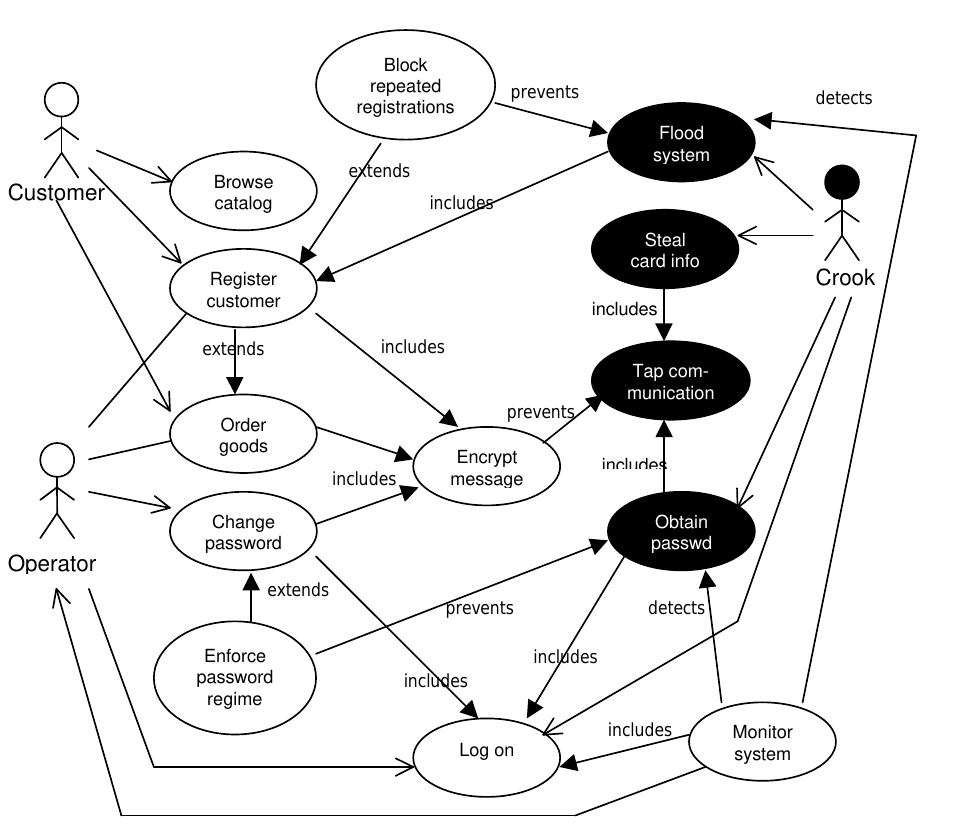
\includegraphics[width=\textwidth, height=0.5\textheight, keepaspectratio]{figures/misusecase.png}
\end{figure}

\FloatBarrier
\subsection{ISO 27000-as család}
\subsubsection{ISO 27001:2013}
Ellentétben a korábbi megközelítésekkel, az \emph{ISO 27001}-es szabvány 

Habár elsőre nem tűnik indokoltnak a megemlítése, elég csupán arra gondolnunk, hogy egy termék
fejlesztésekor elvárhatjuk, hogy a belső infrastruktúránk biztonságos.  Ahogy a cég (és ezzel együtt
az infrastruktúra) növekszik, egyre inkább fontossá válik egy olyan kész keret bevezetése, amelyet
felhasználva biztonságosabb rendszert építhetünk.

\subsection{Common Criteria}

\section{Miért választottuk a Common Criteria-t}

Végeredményként az alábbi metodologiákat kezdtük el alkalmazni:
\begin{itemize}
\item Common Criteria-t a 
\item{ISO 27001:2013-at az infrastruktúra (beleértve a számunkra releváns fejlesztői infrastruktúra)
    biztonságának erősítésére.}
\end{itemize}

A fő okok az alábbiak voltak:

\todo[inline]{Okok listázása}

\section{Common Criteria-ról bővebben}

\subsection{Terminológia}

A későbbiekben előforduló rövidítések itt kerülnek feloldásra.

\begin{description}
    \item[TOE]{Target of Evaluation - az az entitás, amelyre a \emph{Common Criteria} által
            megfogalmazott követelmények teljesülését vizsgáljuk. Esetünkben ez a \emph{syslog-ng}-re,
        mint szoftvercsomagra vonatkozik.}
    \item[EAL]{Evaluation Assurance Level - a követelmények szigorúságának számszerűsített értéke,
        lásd később.}
\end{description}

\subsection{Evaluation Assurance Levels}

Az \emph{Evaluation Assurance Level} (továbbiakban: EAL) egy egytől hétig tartó skálán egyre nagyobb
nyújt, pontosabban a magasabb szinteknél szigorúbb elvárásoknak kell megfelelni. A szigorúbb
elvárásoknak való megfelelőség óhatatlanul magasabb költségekkel is járhat, így az elérni kívánt
szint meghatározásánál figyelembe kell venni, hogy milyen előnyökkel és költségekkel jár annak
elérése. \cite{DipPortal}

\subsubsection{EAL1: funkcionálisan tesztelt}
\todo[inline]{Célja}
\todo[inline]{Miben több, mint az EAL0?}

\subsubsection{EAL2: strukturálisan tesztelt}
\todo[inline]{Célja}
\todo[inline]{Miben több, mint az EAL1?}

\subsubsection{EAL3: metodilikusan tesztelt és ellenőrzött}
\todo[inline]{Célja}
\todo[inline]{Miben több, mint az EAL2?}
\subsubsection{EAL4: }
\todo[inline]{Célja}
\todo[inline]{Miben több, mint az EAL3?}
\subsubsection{EAL5:}
\todo[inline]{Célja}
\todo[inline]{Miben több, mint az EAL4?}
\subsubsection{EAL6:}
\todo[inline]{Célja}
\todo[inline]{Miben több, mint az EAL5?}
\subsubsection{EAL7:}
\todo[inline]{Célja}
\todo[inline]{Miben több, mint az EAL6?}
